%!TEX root = chapter-experiment.tex
\section{Recognition Performance}
\label{sec:experiment:recognition}

We next carried out the 3D palmprint classification and recognition experiments using the first sample of each class in the training database as a template and the 4000 samples in the testing database as probes, making a total of 400 templates and 4000 probes. The performance of classification and recognition is usually measured by error rate and penetration rate calculated in ~\cite{Maltoni:wn} as follows

\begin{equation}
\text{error rate} = \frac{\text{number of false match}}{\text{total number of probe}} \times 100\%
\end{equation}

\begin{equation}
\text{penetration rate} = \frac{\text{number of accessed template}}{\text{total number of template in the database}} \times 100\%
\label{eq:experiment:prate}
\end{equation}

Obviously there is a trade-off between error rates and penetration rates. Generally speaking, if there is no classification, there are two retrieval strategies:

\begin{enumerate}
\item all of the templates in the database are visited and the template that gives the best matching score is regarded as the matched template, if the matching score is less than a given threshold $\Psi_T$
\item given a threshold $\Psi_T$, the search continues until a match is found that is below that threshold
\end{enumerate}

Three 3D palmprint recognition matching approaches are used

\begin{enumerate}
\item no classification
\item coarse-level matching
\item RSVM
\end{enumerate}

For no classification, we matched using the local feature MCI as described in ~\cite{Zhang:2009dp}. The process we used for coarse-level matching is illustrated in Section ~\ref{sec:methodology:featurematch} and involves fine-level matching using the local feature MCI. A single instance of coarse-level matching requires only $1/36000$ of the time it takes to do fine-level matching (coarse-level matching only needs 15 operations while fine-level matching must do $128\times128\times(8\times4+1)$ operations, where $128\times128$ is the size of ROI and $8\times4+1$ is the number of times the template is shifted plus the original unshifted case). For the above two approaches, the penetration rate and the error rate will vary with different thresholds $\Psi_t$. As for RSVM, we use the RSVM algorithm described in Section ~\ref{ssec:methodology:svm} to rank the templates in the database, and then match the top $\rho$ percent by local feature MCI with the best matching score regarded as the matched template if this score is less than a given constant threshold $\Psi_T$. We can see from ~\ref{eq:experiment:prate} that $\rho$ is equal to the penetration rate. Given different thresholds $\Psi_t$ and $\rho$, we carried out a series of 3D palmprint recognition experiments.

% Table generated by Excel2LaTeX from sheet 'Sheet1'
\begin{table}[htbp]
  \centering
  \caption{Penetration rate and error rate with no classification}
    \begin{tabular}{cc}
    \toprule
    Penetration rate (\%) & Error rate (\%) \\
    \midrule
    100  & 1.29 \\
    51.1  & 1.68 \\
    49.3  & 1.86 \\
    47.2  & 2.1 \\
    45.9  & 2.33 \\
    43.7  & 2.6 \\
    42.6  & 2.95 \\
    41.5  & 3.3 \\
    40.3  & 3.75 \\
    38.1  & 4.8 \\
    35.9  & 5.86 \\
    \bottomrule
    \end{tabular}%
  \label{tab:experiment:noclass}%
\end{table}%

% Table generated by Excel2LaTeX from sheet 'Sheet1'
\begin{table}[htbp]
  \centering
  \caption{Penetration rate and error rate using coarse-level matching}
    \begin{tabular}{|c|c|}
    \hline
    Penetration rate (\%) & Error rate (\%) \\
    \hline
    45.2  & 1.31 \\ \hline
    41.6  & 1.32 \\ \hline
    38.8  & 1.36 \\ \hline
    34.7  & 1.42 \\ \hline
    29.1  & 1.56 \\ \hline
    23.5  & 1.78 \\ \hline
    20.5  & 2.12 \\ \hline
    18.4  & 2.39 \\ \hline
    13.3  & 3.16 \\ \hline
    10.1  & 4.3 \\ \hline
    8.6   & 5.79 \\
    \hline
    \end{tabular}%
  \label{tab:experiment:coarse}%
\end{table}%

% Table generated by Excel2LaTeX from sheet 'Sheet1'
\begin{table}[htbp]
  \centering
  \caption{Penetration rate and error rate using RSVM}
    \begin{tabular}{|c|c|}
    \hline
    Penetration rate (\%) & Error rate (\%) \\
    \hline
    30    & 1.3 \\ \hline
    27.5  & 1.33 \\ \hline
    25    & 1.37 \\ \hline
    22.5  & 1.42 \\ \hline
    20    & 1.49 \\ \hline
    17.5  & 1.63 \\ \hline
    15    & 1.87 \\ \hline
    12.5  & 2.48 \\ \hline
    10    & 3.35 \\ \hline
    7.5   & 4.41 \\ \hline
    5     & 5.88 \\
    \hline
    \end{tabular}%
  \label{tab:experiment:svm}%
\end{table}%


Table ~\ref{tab:experiment:noclass}, ~\ref{tab:experiment:coarse} and ~\ref{tab:experiment:svm} difference in penetration rate and error rate using different recognition strategies. Even at an approximately equal error rate, the proposed coarse-level matching and RSVM approaches get a much lower penetration rate than the no classification approach. Obviously RSVM has the best performance but requires an additional off-line training process compared to coarse-level matching.

\begin{figure}[htb]
\begin{center}
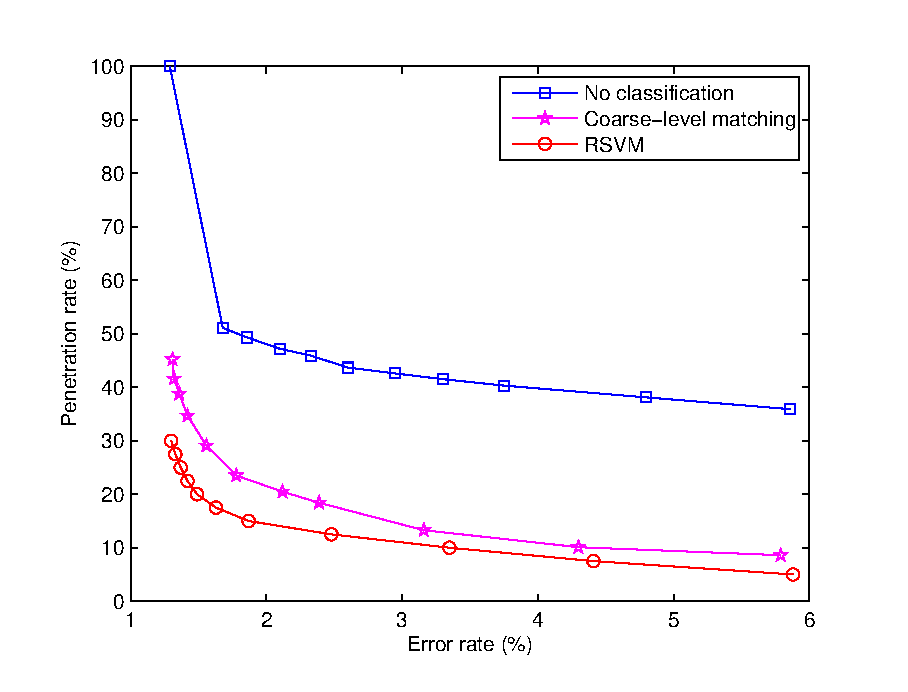
\includegraphics[width=\linewidth]{ch-experiment/figures/recognition}
\caption{Penetration rate and error rate with different matching strategies}
\label{fig:experiment:recognition}
\end{center}
\end{figure}

Figure ~\ref{fig:experiment:recognition} shows the results in a single plot.

% Table generated by Excel2LaTeX from sheet 'Sheet2'
\begin{table}[htbp]
  \centering
  \caption{Running time comparison of the three 3D palmprint recognition approaches}
    \begin{tabular}{lrrr}
    \toprule
          & No classification & Coarse-level matching & RSVM \\
    \midrule
    \multicolumn{1}{p{5cm}}{Once feature extraction time} & 112ms & 136ms & 136ms \\
    \multicolumn{1}{p{5cm}}{Once dimensionality reduction time} & 0ms   & 0.1ms & 0.1ms \\
    \multicolumn{1}{p{5cm}}{Ranking or coarse matching time for all templates in database} & 0ms   & 0.5ms & 1.56ms \\
    \multicolumn{1}{p{5cm}}{Once matching time by MCI} & 0.86ms & 0.86ms & 0.86ms \\
    \multicolumn{1}{p{5cm}}{Total running time for one probe testing} & 456ms & 292.09ms & 240.86ms \\
    \bottomrule
    \end{tabular}%
  \label{tab:experiment:time}%
\end{table}%



Table ~\ref{tab:experiment:time} shows the difference in time consumption for one probe. Due to the lower penetration rate, the running times are greatly reduced.
